
\chapter{Anforderungen an die Web-Applikation}

\section{Spotbeschreibungen}

Eine der bekanntesten Wellen in Europa ist im spanischen Baskenland an
einer Fluss\-mündung östlich des Ortes \textit{Mundaka} zu finden. Im
\textit{Stormrider Guide Europe} \cite[S.180]{storm_europe_1998}
werden die Surfbedingungen an diesem Spot wie folgt beschrieben.

\vspace{0.2cm}

\textit{Some of the longest, hollowest lefts in Europe break over
  sandbanks at the mouth of the river Gernike. It's best at low tide,
  when the rivers current (a useful conveyor belt) is less intense,
  and holds swell up to 4m (12ft). On the other side of the rivermouth
  are the beaches Laida and Laga where you can find waves at small
  swells. The river and its estuary are a Worldwide Fund for Nature
  reserve, but even so, the water is not as clean as could expected.
}

\vspace{0.2cm}

Zusätzlich werden den Beschreibungen Piktogramme aus verschiedenen
Kategorien zugeordnet, welche die Gegebenheiten vor Ort durch eine
vereinfachte grafische Darstellung widerspiegeln. Einige dieser
Kategorien sind die bevorzugte Windrichtung, die optimale Gezeit, die
Art der brechenden Welle, Beschaffenheit des Bodens sowie mögliche
Gefahren. Durch die Piktogramme ist mit einem kurzen Blick schnell
ersichtlich, welche Bedingungen an einem Spot herrschen. In Abbildung
\ref{piktogramm} sind die Piktogramme zu sehen, die für die obige
Beschreibung in Mundaka verwendet wurden. Sie sollen vermitteln, dass
dieser Spot sehr bekannt ist und an guten Tagen mit vielen Surfern zu
rechnen ist. Die Welle bricht mit viel Kraft von links nach rechts
(\textit{Left-hander}, immer vom Strand aus gesehen) über einer
Sandbank, wobei vereinzelt Surfbretter zu Bruch gehen können.  Sie ist
nicht bei Flut (\textit{High Tide}) surfbar, und ablandiger Wind
(\textit{Offshore}) aus dem Süden trägt dazu bei, dass die Wellen
geglättet werden, später brechen und hohler werden.

\begin{figure}[t]
  \begin{center}
    
\includegraphics[height=40px]{bilder/mundaka-conditions}
    \caption{Piktogramme zu den Surfbedingungen in Mundaka}
    \label{piktogramm}
  \end{center}
\end{figure}

Das Konzept der Stormrider Guides soll die Grundlage der Web
Applikation bilden und mit den Möglichkeiten des Internets verknüpft
werden. Die Beschreibungen zu den Spots und deren Gegebenheiten sollen
gemeinschaflich durch die Mitglieder der Surf Community verfasst
werden, und als sogenannter \textit{User Generated Content} verwaltet
werden. Die gemeinsam erstellten Beschreibungen sollen eine objektive
Sicht auf die Gegebenheiten und Surfbedingungen an den jeweiligen
Spots bieten. Für persönliche Ansichten und Diskussionen werden
zusätzlich Kommentarfunktionen zur Verfügung gestellt. Um Spam und
anderer mutwilliger Zerstörung oder Verunreinigung des Contents
vorzubeugen, ist für bestimmte Funktionen eine Registrierung der
Nutzer erforderlich. Für alle Informationen, die gemeinschaftlich von
Nutzern der Web-Applikation verändert werden können, soll eine
Historie verwaltet werden. Dadurch soll sichergestellt werden, dass
bei einer eventuellen Verunreinigung des Contents auf eine frühere
Version der Information zurückgegriffen und der ursprüngliche Zustand
wieder hergestellt werden kann.

\section{Kartenmaterial}

Um das Auffinden von Spots zu vereinfachen, sollen diese auf einer
Karte dargestellt werden. Webservice-Dienste wie \textit{Google Maps},
\textit{Yahoo! Maps} oder Microsoft's \textit{Bing Maps}
\footnote{seit Juni 2009, früher: Microsoft's Virtual Earth} bieten
die Möglichkeit, interaktive Karten per Java\-script oder Flash in
eine Webseite einzubetten. Diese Dienste bieten nicht nur die
typischen Land- bzw. Straßenkarten an, sondern stellen auch
Satelitenbilder und teilweise dreidimensionale Ansichten für bestimmte
Gebiete zur Verfügung. In Abbildung \ref{google-maps} ist eine Karten-
und eine Satellitenansicht von dem Surfspot in \textit{Mundaka} zu
sehen. Insbesondere die Satellitenansicht ist beim Auffinden von neuen
oder geheimen Surfspots recht nützlich, da man darauf sehr gut
brechende Wellen erkennen und sich einen Überblick auf das Gelände
verschaffen kann.

\begin{figure}[h]
  \subfigure[Karten Ansicht]{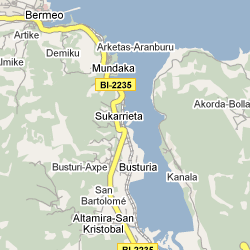
\includegraphics[width=0.49\textwidth]{bilder/google-maps-map}}
  \subfigure[Satelliten Ansicht]{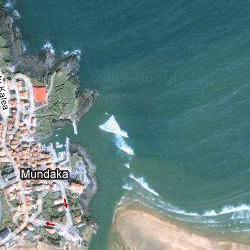
\includegraphics[width=0.49\textwidth]{bilder/google-maps-hybrid}}
  \caption{\textit{Google Maps} Kartenmaterial für Mundaka, Spanien}
  \label{google-maps}
\end{figure}

\section{Wetter- und Wellendaten}
\label{sec:Wetter- und Wellendaten}

Wie schon in der Einleitung erwähnt, ist das Vorhandensein von Swell
eine der Grundvoraussetzungen zum Surfen. Viele Surfer nutzen deshalb
regelmäßig Dienste im Internet, um sich über die Wetter- und
Wellenverhältnisse in den nächsten Tagen zu informieren. Dabei ist
hauptsächlich die Wellenhöhe, die Wellenperiode sowie die Stärke und
die Richtung des Windes von Interesse. Die Spotbeschreibungen sollen
deshalb mit aktuellen Wetter- und Wellenvorhersagen verknüpft werden,
um den Benutzern der Web-Applikation einen Ausblick auf die
Surfbedingungen in den nächsten Tagen bieten zu können. Die
\textit{National Oceanic and Atmospheric Administration (NOAA)} ist
die Wetter- und Ozeanografiebehörde der Vereinigten Staaten. Sie
besteht aus 5 größeren Organisationen, zu denen unter anderen auch der
\textit{National Weather Service (NWS)} \nomenclature{NWS}{National
  Weather Service} und der \textit{National Ocean Service (NOS)}
\nomenclature{NOS}{National Ocean Service} gehören, welche die
benötigten Wetter- und Wellendaten zur Verfügung stellen. Viele der im
Internet verfügbaren Dienste, die Wetter- oder Wellenvorhersagen
anbieten, beziehen ihre Daten ebenfalls von diesen
Organisationen. Diese Vorhersagen sind zwar insbesondere an
Küstengegenden nicht sehr genau, tragen aber einen wichtigen Teil dazu
bei, die Surfbedingungen in einer bestimmten Region oder an einem Spot
grob einzuschätzen zu können.

\begin{figure}[h]
 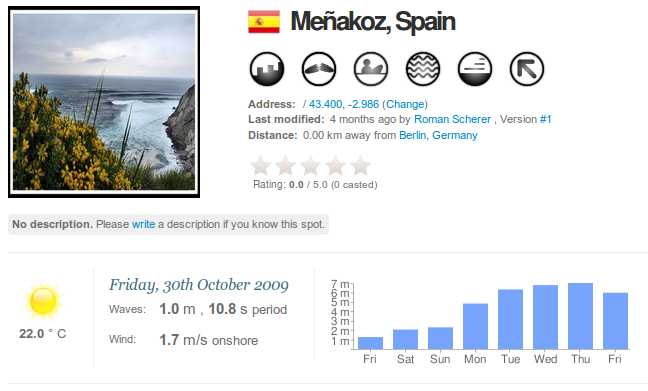
\includegraphics[width=\textwidth]{bilder/forecast}
 \caption{Wetter- und Wellenvorhersage für Meñakoz, Spanien}
 \label{forecast}
\end{figure}

\section{Bilder \& Videos}
Um Surfern einen visuellen Eindruck der Spots bieten zu können, sollen
diese mit Bildern und Videos verknüpft werden. Diese in der Surf
Community gerne gesehenen Bilder und Videos sind ideal um das bisher
aus Beschreibungen, Wetter- und Wellenvorhersagen bestehende
Informationsangebot aufzuwerten. Zum einen sollen externe Bilder und
Videos durch die Nutzung von \textit{Web Services} in die Applikation
integriert werden, und zum anderen den Nutzern die Möglichkeit gegeben
werden, ihre eigenen Bilder und Videos auf der Plattform zu
publizieren.

\subsubsection{Integration externer Bilder und Videos}
Auf Internetseiten wie \textit{Flickr} und \textit{YouTube} sind von
vielen bekannten Spots Bilder und Videos zu finden. Eine Suchanfrage
nach einem bekannten Spot mit den Stichwörtern \textit{Mavericks} und
\textit{Surf} ergab im Juni 2009 bei \textit{Flickr} 2319 und bei
\textit{YouTube} 548 Ergebnisse. Die Integration diese externen
Informationen ist insbesondere im Anfangsstadium der Web-Applikation
nützlich, da in dieser Phase noch wenig Content durch die Nutzer
generiert wurde. Durch Einbindung externer Bilder und Videos kann
somit die Qualität des gesamten Content verbessert werden. Sowohl
\textit{Flickr} als auch \textit{YouTube} bieten zur Integration Web
Service Schnittstellen an, mit denen es möglich ist deren Bilder und
Videos in eigene Anwendungen zu integrieren.

\begin{figure}[h]
 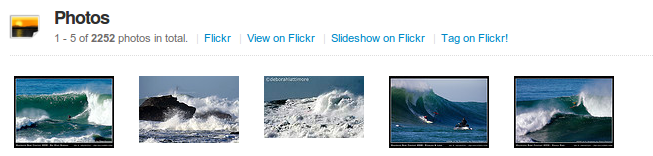
\includegraphics[width=\textwidth]{bilder/photos-flickr}
 \caption{Integration von Bildern durch den \textit{Flickr}
      Webservice}
 \label{photos-flickr}
\end{figure}

\subsubsection{Publikation eigener Bilder und Videos}
Zudem soll den Nutzern die Möglichkeit gegeben werden, ihre eigenen
Bilder und Videos auf die Community-Plattform zu laden und diese dort
zu veröffentlichen. Im Moment wird genau diese Funktionalität mit
großem Erfolg zwar auch von \textit{Flickr} und \textit{YouTube}
angeboten, aber mit Blick auf zukünftige Erweiterungen ist es
sinnvoll, die volle Kontrolle über die auf der Plattform angezeigten
Bilder und Videos zu haben. Der Einbau eines Abstimmungssystems und
ähnlicher Funktionen kann mit externen Abhängigkeiten schnell
problematisch werden und soll deshalb vermieden werden. Um das vor
allem durch Videos erhöhte Datenvolumen in den Griff zu bekommen,
werden Bilder und Videos auf \textit{Amazon's Simple Storage Service
  (S3)} \footnote{http://aws.amazon.com/s3} gehostet. Dadurch können
Probleme wie mangelnder Speicherplatz, Skalierbarkeit und hohe
Verfügbarkeit der Daten ausgelagert werden und zugleich die
Komplexität beim Deployment der Plattform reduziert werden.

\begin{figure}[h]
 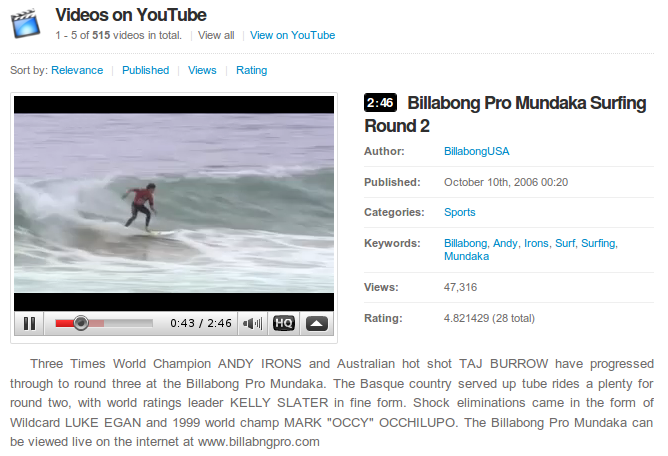
\includegraphics[width=\textwidth]{bilder/youtube}
 \caption{Integration von Videos durch den \textit{YouTube}
      Webservice}
 \label{youtube}
\end{figure}

\section{Community-Funktionen}
Community-Plattformen wie \textit{Facebook}, \textit{MySpace} und
\textit{StudiVZ} erfreuen sich in den letzten Jahren einer sehr großen
Beliebtheit. Einige der dort bewährten Funktionalitäten sind auch in
der hier entwickelten Web-Applikation sinnvoll und könnten einen
Beitrag dazu leisten, den Nutzern einen Mehrwert zu bieten und sie
enger an die Plattform zu binden. Beispielsweise sollen die gemeinsam
erstellten Spotbeschreibungen, die eine objektive Sicht auf einen Spot
darstellen, mit den subjektiven Kommentaren und Meinungen der Nutzer
verknüpft werden, um eine Diskussion zu ermöglichen. Auf der Plattform
publizierte Bilder und Videos sollen ebenfalls kommentiert und
bewertet werden, damit diese nach verschiedenen Kriterien wie
Relevanz, Beliebtheit usw. sortiert und angezeigt werden können. Damit
die Plattform lebendiger wird, können Nutzer ihr eigenes Profilbild
verwalten und Freundschaften mit anderen Nutzern eingehen. Darauf
aufbauend soll es möglich sein, sowohl private als auch öffentliche
Nachrichten an andere Nutzer zu senden und in den freigegebenen
Profilseiten der registrierten Surfer zu stöbern. Um die Privatsphäre
der Nutzer zu respektieren, müssen einige diese Funktionen von den
Anwendern freigeschalten bzw. gesperrt werden können. Einige dieser
Konzepte werden zwar von vielen als ''Spielerei'' angesehen, für
andere sind dies aber einige der Gründe, eine Community-Plattform zu
nutzen und tragen wohl auch einen großen Teil zum Erfolg vieler
bereits etablierter Community-Plattformen bei.

\section{Nachhaltiges Publizieren}
Ein relativ unschönes, aber teilweise auch verständliches Phänomen in
der Surfszene ist der sogenannte Lokalismus oder \textit{Localism} im
Englischen. Entgegen dem allgemeinen Klischee, dass Surfer friedliche
und entspannte Menschen sind, wird dieser Eindruck an einigen Spots
durch unsportliches Verhalten einiger weniger getrübt. Beim Surfen
bekommt meist derjenige die Welle, der sie am schnellsten anpaddelt,
sich die bessere Technik antrainiert hat und am meisten Erfahrung
hat. Kurz gesagt, der Stärkere. Bei guten Surfbedingungen mit vielen
Leuten führt dies unweigerlich dazu, dass einige Surfer die Wellen
fast immer und andere fast nie bekommen. Insbesondere an Wochenenden
und Feiertagen, an denen viele Surfer ihrem Hobby nachgehen, sind
viele Spots überfüllt und es kann zu aggressivem Verhalten auf dem
Wasser kommen.

\begin{figure}[h]
  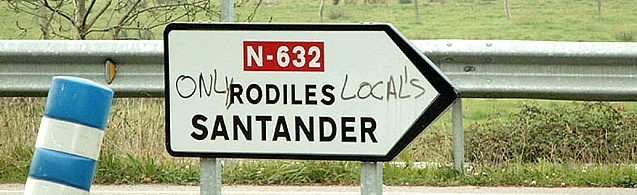
\includegraphics[width=\textwidth]{bilder/locals-only}
  \caption{\textit{''Only Rodiles Locals''} - Lokalismus in Rodiles,
    Spanien}
  \label{locals-only}
\end{figure}

Vor Ort ansässige Surfer, sogenannte \textit{Locals}, fühlen sich
teilweise durch die vielen Besucher an ''ihren'' Spots bedrängt und
reagieren auf diese mit aggressivem Verhalten. Wie in Abbildung
\ref{locals-only} zu sehen ist, wird fremden Surfern deshalb oft durch
Grafittis oder ähnliche Markierungen nahe gelegt, dass sie an einem
Spot nichts zu suchen haben. Dies gelingt teilweise auch, da es
zuweilen vorkommt, dass man einen Spot mit einem unguten Gefühl
besucht. Grundsätzlich gilt deshalb, je weniger Surfer an einem Spot
sind, desto entspannter ist die Atmosphäre und desto eher kommt jeder
auf seine Kosten. Abgelegenere oder nur schwer zugängliche Spots
werden deshalb von \textit{Locals} oft als geheim gehandelt, gegenüber
Fremden nicht erwähnt oder diese beim Suchen nach Spots in die Irre
geführt.

Um die vor Ort ansässigen Surfer zu respektieren und nicht sofort
jeden neuen Spot in die Welt hinaus zu posaunen, wurde hier deshalb
das Konzept der \textit{Secret Spots} eingeführt. Auf der Plattform
sollen nur die allgemein bekannten Spots für jeden sichtbar
sein. Diese Spots befinden sich meist an bekannten Stränden, sind
ausgeschildert und auch in den Karten vieler Tourismusbüros
verzeichnet. Andere Spots können beim Erstellen als \textit{Secret
  Spots} markiert werden und sind dann nur für den Ersteller selbst
und eingeladene Freunde sichtbar. Alle anderen Funktionen, wie Wetter-
und Wellenvorhersagen stehen für diese Spots ebenfalls zur Verfügung,
allerdings nur für einen eingeschränkten Nutzerkreis.

\begin{figure}[t]
 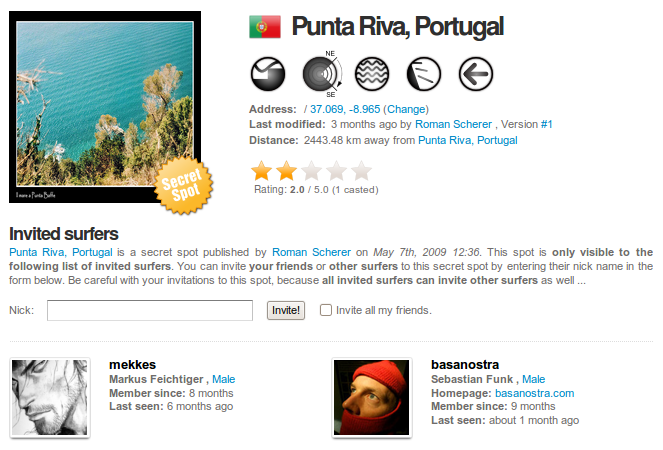
\includegraphics[width=\textwidth]{bilder/secret-spot}
 \caption{Ansicht der Einladungen zu einem Secret Spot}
 \label{secret-spot}
\end{figure}

%%% Local Variables:
%%% mode: latex
%%% TeX-master: "../community-plattform"
%%% End:
